\documentclass[12pt,titlepage]{article}
\usepackage[margin=1.25in]{geometry}
\usepackage{graphicx,amsmath,blindtext,minted}

%% Variables definition
\newcommand{\vSubject}{Web Design and Development}
\newcommand{\vSubtitle}{PHP Form Proccessing}
\newcommand{\vName}{Muhammad Baihaqi Aulia Asy'ari}
\newcommand{\vNIM}{2241720145}
\newcommand{\vClass}{2I}
\newcommand{\vDepartment}{Information Technology}
\newcommand{\vStudyProgram}{D4 Informatics Engineering}

%% [START] Tikz related stuff
\usepackage{tikz}
\usetikzlibrary{svg.path,calc,shapes.geometric,shapes.misc}
\tikzstyle{terminator} = [rectangle, draw, text centered, rounded corners = 1em, minimum height=2em]
\tikzstyle{preparation} = [chamfered rectangle, chamfered rectangle sep=0.75em, draw, text centered, minimum height = 2em]
\tikzstyle{process} = [rectangle, draw, text centered, minimum height=2em]
\tikzstyle{decision} = [diamond, aspect=2, draw, text centered, minimum height=2em]
\tikzstyle{data}=[trapezium, draw, text centered, trapezium left angle=60, trapezium right angle=120, minimum height=2em]
\tikzstyle{connector} = [line width=0.25mm,->]
%% [END] Tikz related stuff

%% [START] Fancy header related stuff
\usepackage{fancyhdr}
\pagestyle{fancy}
\setlength{\headheight}{15pt} % compensate fancyhdr style
\fancyhead{}
\fancyfoot{}
\fancyfoot[L]{\thepage}
\fancyfoot[R]{\textit{\vSubject - \vSubtitle}}
\renewcommand{\footrulewidth}{0.4pt}% default is 0pt, overline for footer
%% [END] Fancy header related stuff

%% [START] Custom tabular command related stuff
\usepackage{tabularx}
\newcommand{\details}[2]{
    #1 & #2  \\
}
%% [END] Custom tabular command related stuff

%% [START] Figure related stuff
\newcommand{\image}[3][1]{
    \begin{figure}[h]
        \centering
        \includegraphics[#1]{#2}
        \caption{#3}
        \label{#3}
    \end{figure}
}
%% [END] Figure related stuff

%%
\usepackage{pgf-umlcd}

\renewcommand{\umldrawcolor}{black}
\renewcommand{\umlfillcolor}{white}
%%

%% [BEGIN] Custom enumerator
\usepackage{enumitem}
%% [END] Custom enumerator

%% [BEGIN] Paragraph indent
\usepackage{indentfirst}
%% [END] Paragraph indent

%% [BEGIN] enumii
\renewcommand{\labelenumii}{\arabic{enumi}.\arabic{enumii}}
%% [END] enumii

\begin{document}
\begin{titlepage}
    \centering
    \vfill
    {\bfseries\LARGE
        \vSubject\\
        \vskip0.25cm
        \vSubtitle
    }
    \vfill
    
\includegraphics[width=6cm]{images/polinema-logo.png}
    \vfill
    {
        \textbf{Name}\\
        \vName\\
        \vskip0.5cm
        \textbf{NIM}\\
        \vNIM\\
        \vskip0.5cm
        \textbf{Class}\\
        \vClass\\
        \vskip0.5cm
        \textbf{Department}\\
        \vDepartment\\
        \vskip0.5cm
        \textbf{Study Program}\\
        \vStudyProgram
    }
\end{titlepage}

\newpage

\begin{enumerate}
    \item -
    \begin{enumerate}
        \item - \\ 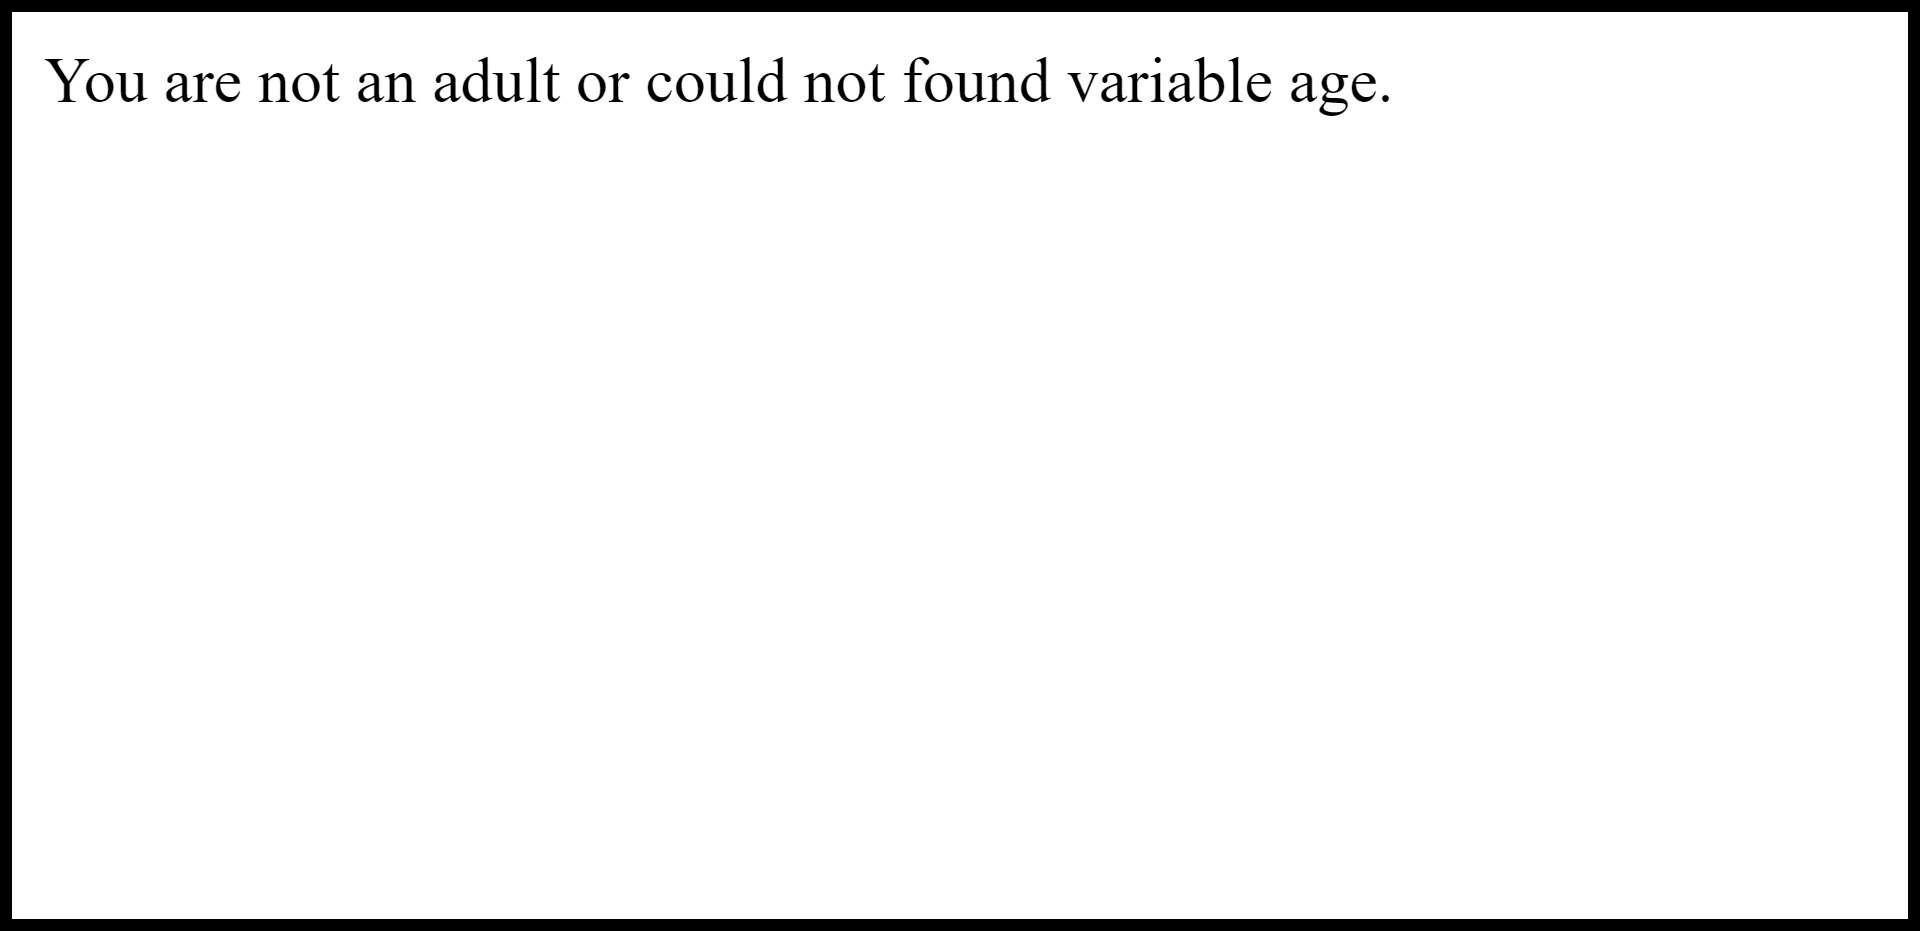
\includegraphics[width=.85\textwidth]{images/figures/fig1.1.png} \\ Isset can check wether or not a variable has been set
        \item - \\ 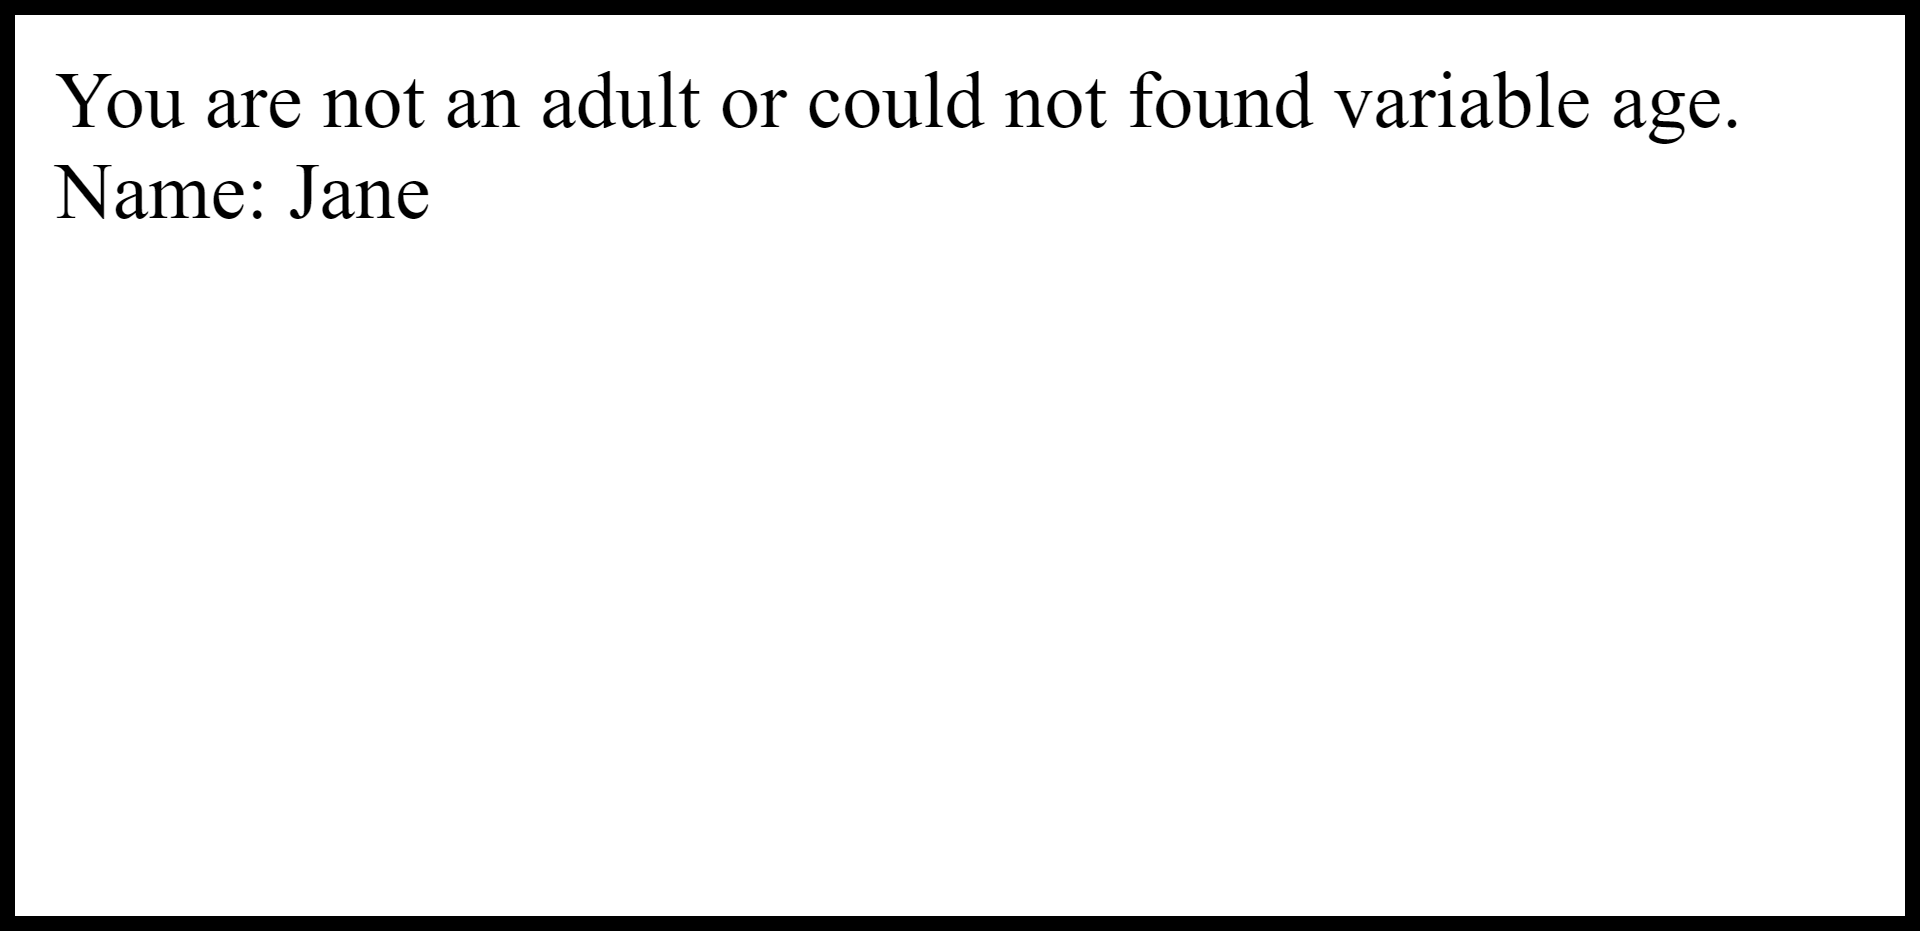
\includegraphics[width=.85\textwidth]{images/figures/fig1.2.png} \\ Isset can check the existence of a value of a certain key in an assosiative array
    \end{enumerate}

    \newpage

    \item -
    \begin{enumerate}
        \item - \\ \includegraphics[width=.85\textwidth]{images/figures/fig2.1.png} \\ The empty() function return a boolean value after checking if the variable in the parameter is empty or not
        \item - \\ \includegraphics[width=.85\textwidth]{images/figures/fig2.2.png} \\ The empty() function return a boolean value after checking if the variable in the parameter is undefined or not
    \end{enumerate}

    \newpage

    \item -
    \begin{enumerate}
        \item - \\ \includegraphics[width=.85\textwidth]{images/figures/fig3.1_a.png} \\ \includegraphics[width=.85\textwidth]{images/figures/fig3.1_b.png} \\ When a post form is submited the action can process the data posted by the form
        
        \newpage
        
        \item - \\ 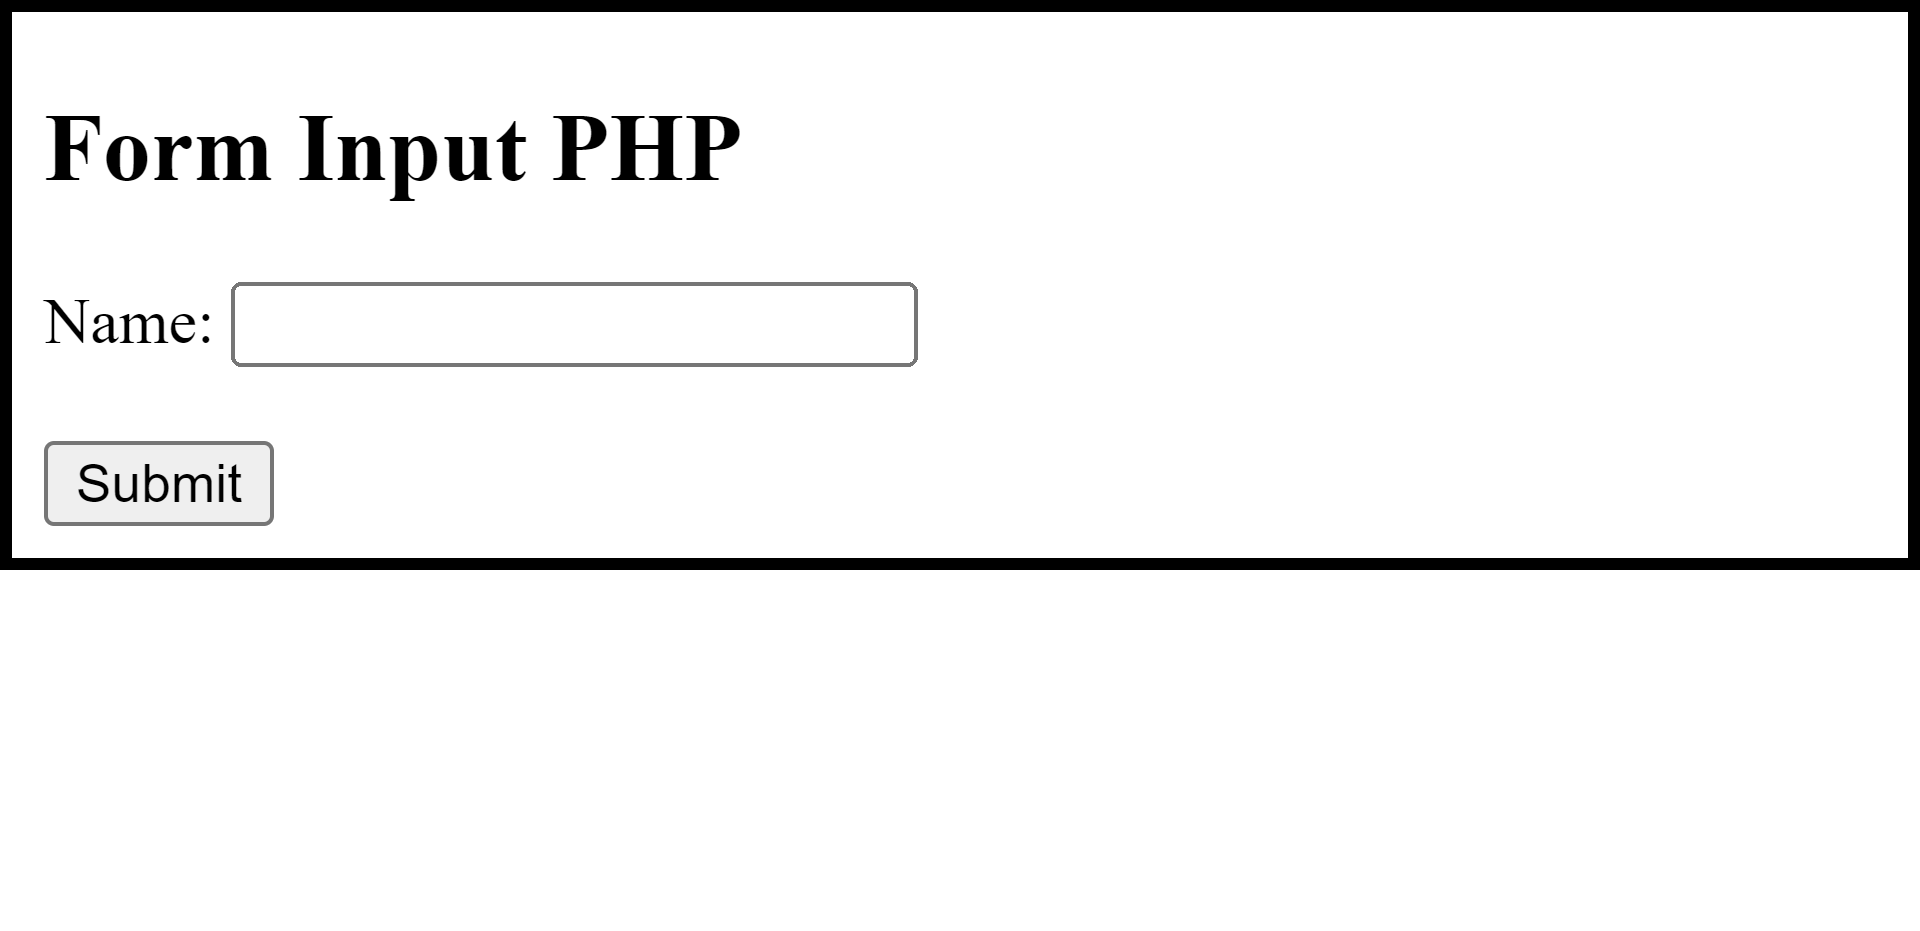
\includegraphics[width=.85\textwidth]{images/figures/fig3.2_a.png} \\ \includegraphics[width=.85\textwidth]{images/figures/fig3.2_b.png} \\ \includegraphics[width=.85\textwidth]{images/figures/fig3.2_c.png} \\ Now when a post form is submited the action call the self php
    \end{enumerate}
    
    \newpage

    \item -
    \begin{enumerate}
        \item -
        \begin{minted}[autogobble,breaklines]{php}
            <!-- // ! Experiment 4 - HTML Injection -->
            <!-- // * 4.1 -->
            <!DOCTYPE html>
            <html>
                <head>
                    <title>Secure HTML</title>
                    <style>
                        html {
                            border: 3px solid black;
                        }
                    </style>
                </head>
                <body>
                    <h2>Secure HTML</h2>
                    <?php
                    $input;
                    if ($_SERVER['REQUEST_METHOD'] == 'POST') {
                        if (empty($input)) {
                            $input = $_POST['input'];
                            $input = htmlspecialchars($input, ENT_QUOTES, 'UTF-8');
                            echo $input;
                        }
                    }
                    ?>
                    <form action="<?php echo htmlspecialchars($_SERVER['PHP_SELF']);?>" method="post">
                        <label for="input">Input:</label>
                        <input type="text" name="input" id="input">
                        <input type="submit" value="Submit">
                    </form>
                </body>
            </html>
        \end{minted}
        
        \newpage

        \includegraphics[width=.85\textwidth]{images/figures/fig4.1_a.png} \\ 
        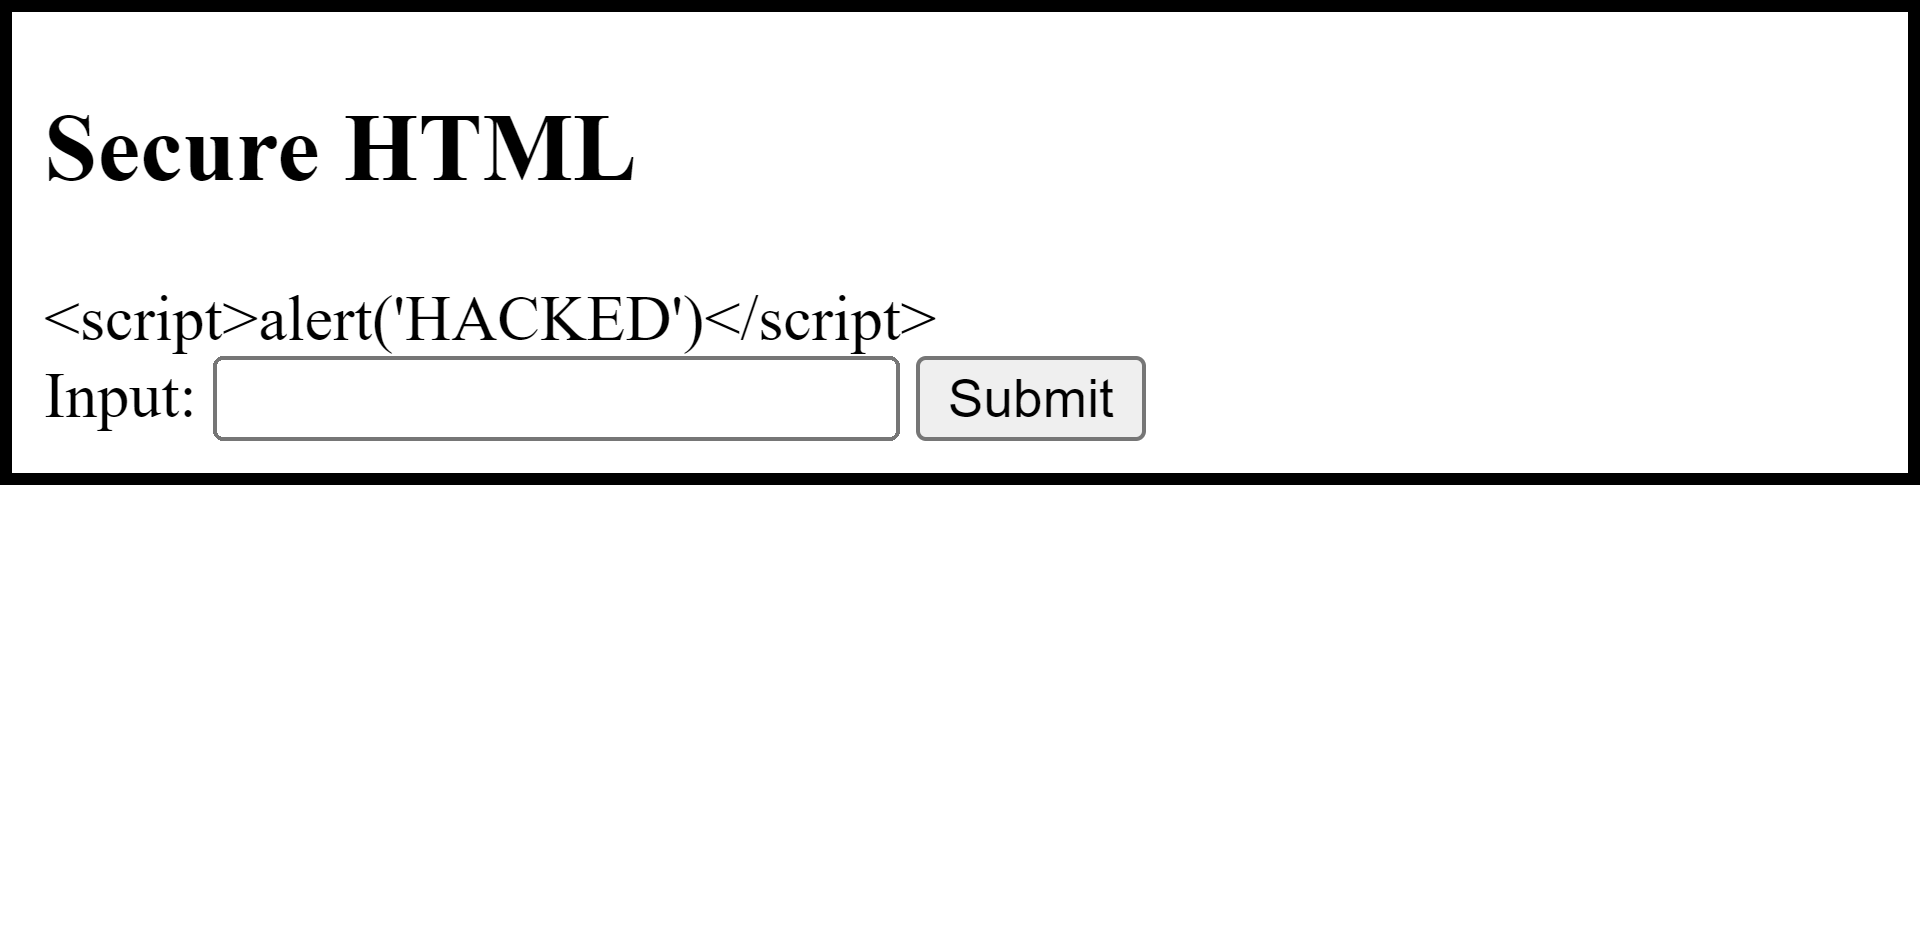
\includegraphics[width=.85\textwidth]{images/figures/fig4.1_b.png} \\ 
        with the htmlspecialchars() function the html is now protected from injection
        
        \newpage

        \item -
        \begin{minted}[autogobble,breaklines]{php}
            <!-- // * 4.2 -->
            <head>
                <title>Secure HTML</title>
                <style>
                    html {
                        border: 3px solid black;
                    }
                </style>
            </head>
            <h2>Secure HTML</h2>
            <?php
            $email;
            if ($_SERVER['REQUEST_METHOD'] == 'POST') {
                $email = $_POST['email'];
                if (isset($input)) {
                    if (filter_var($email, FILTER_VALIDATE_EMAIL)) {
                        echo $email;
                    } else {
                        echo "Email invalid";
                    }
                }
            }
            ?>
            <form action="<?php echo htmlspecialchars($_SERVER['PHP_SELF']);?>" method="post">
                <label for="email">Email:</label>
                <input type="email" name="email" id="email">
                <input type="submit" value="Submit">
            </form>
        \end{minted}

        \newpage

        \includegraphics[width=.85\textwidth]{images/figures/fig4.2_a.png} \\
        \includegraphics[width=.85\textwidth]{images/figures/fig4.2_b.png} \\
        
        \newpage
        
        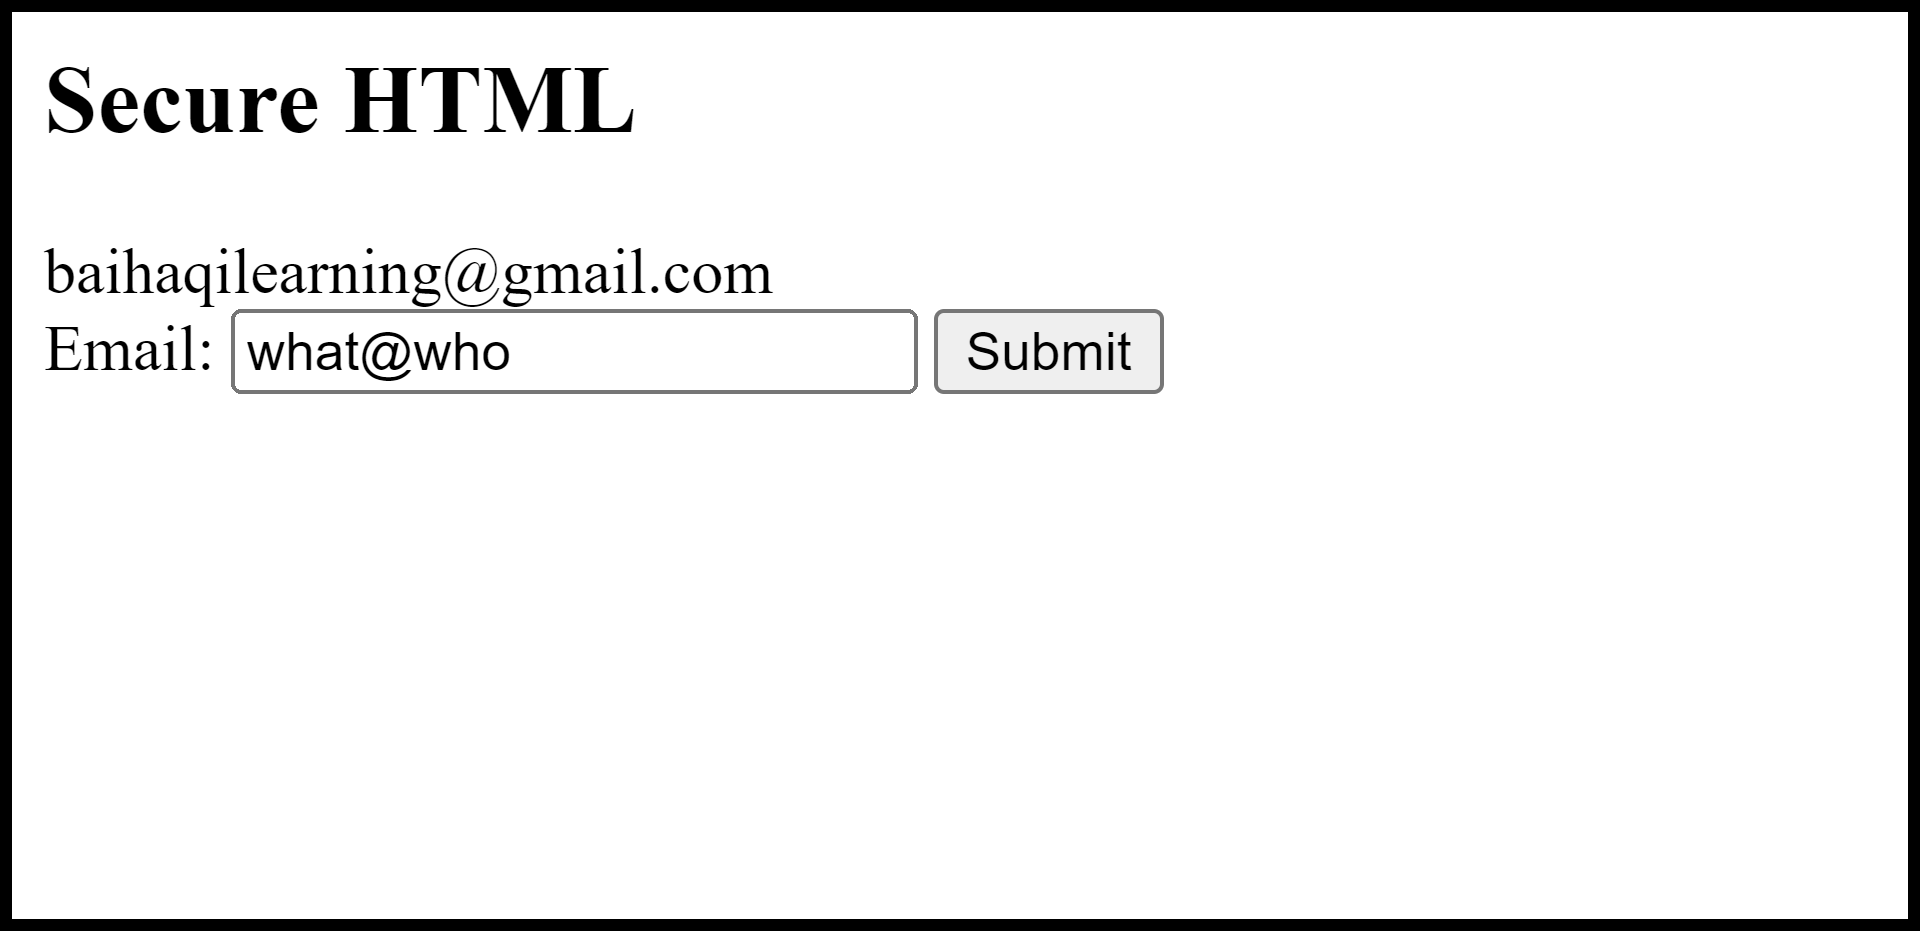
\includegraphics[width=.85\textwidth]{images/figures/fig4.2_c.png} \\
        \includegraphics[width=.85\textwidth]{images/figures/fig4.2_d.png} \\
        If an email is invalid it return false which we can use to print out an error message
    \end{enumerate}

    \newpage

    \item -
    \begin{enumerate}
        \item - \\ 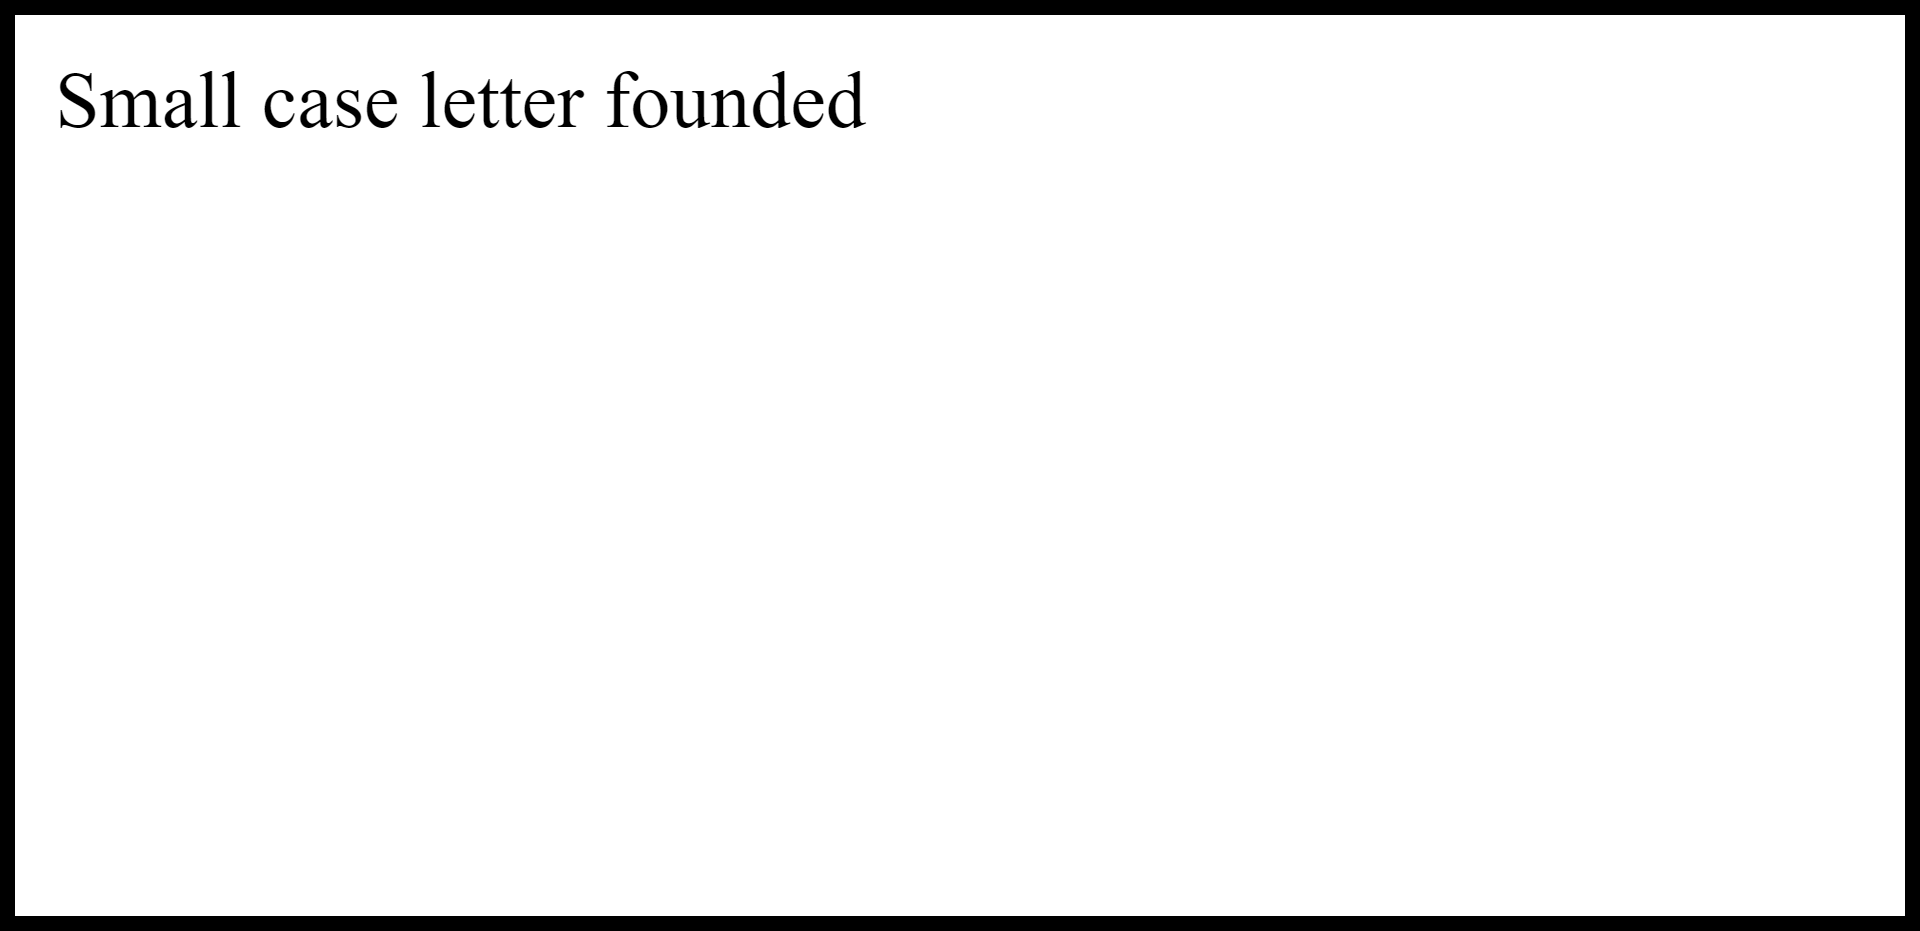
\includegraphics[width=.85\textwidth]{images/figures/fig5.1.png} \\ The RegEx allows us to check whether or not a certain letter or group of letter exist in a variable
        \item - \\ 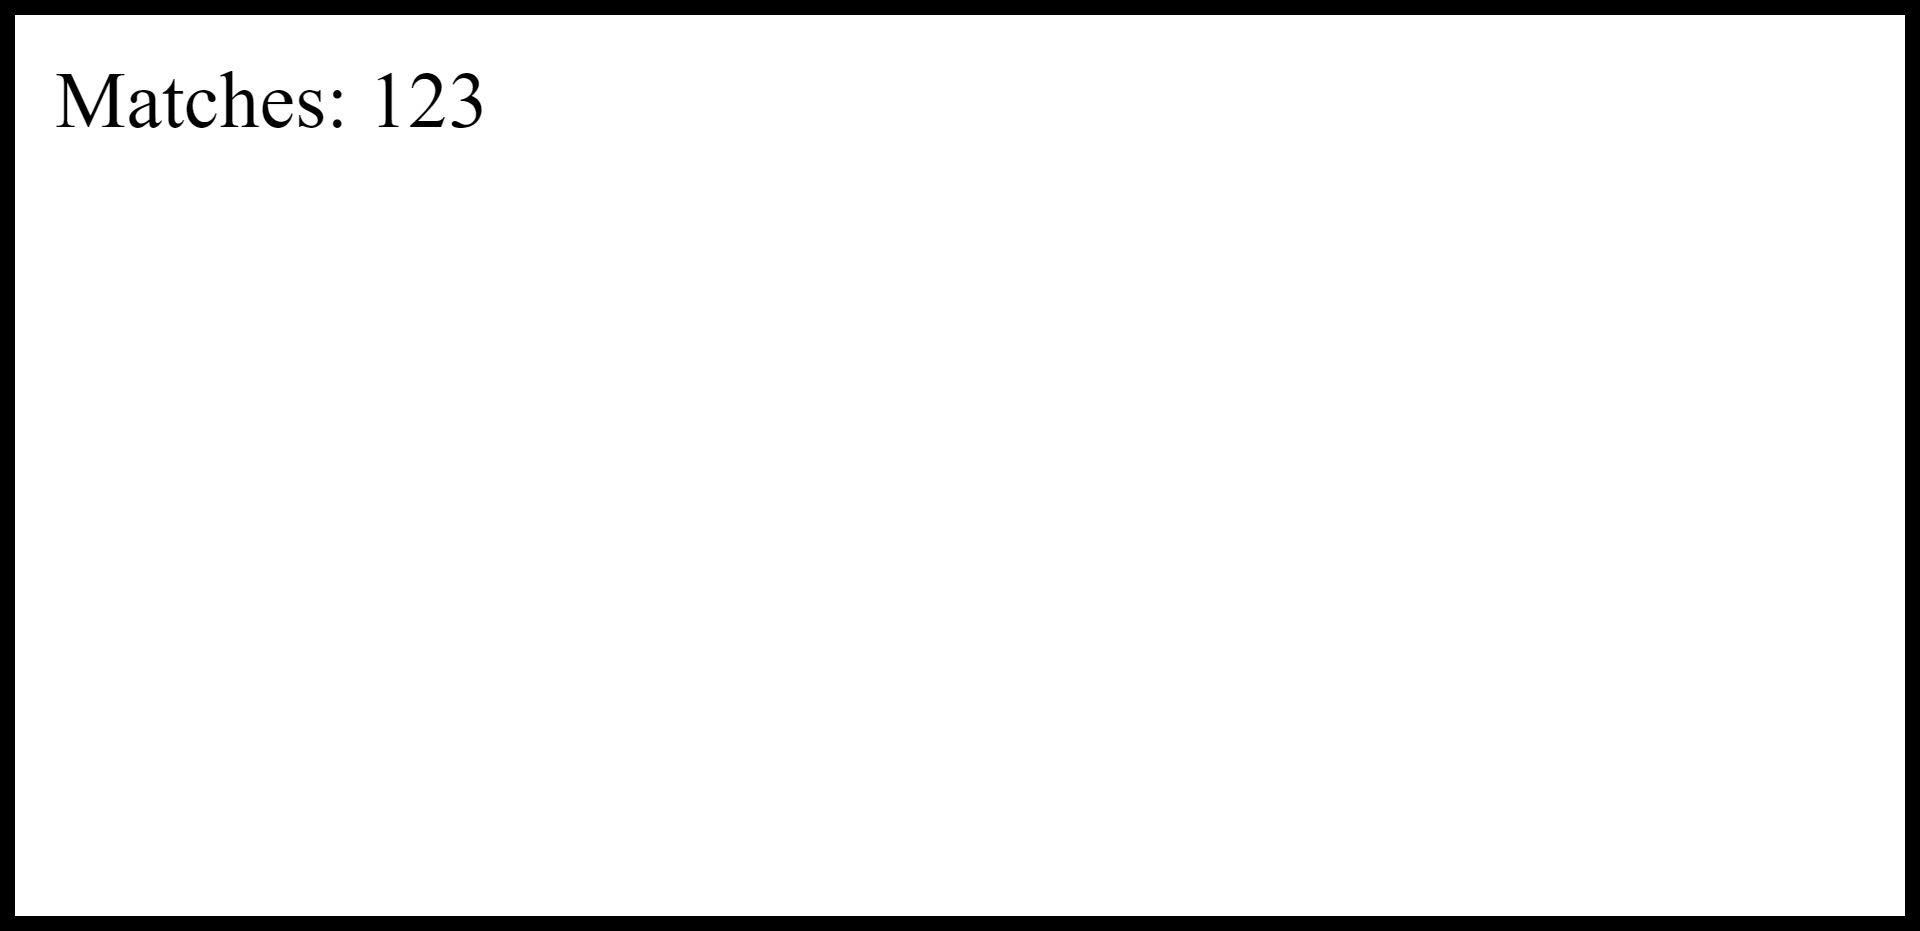
\includegraphics[width=.85\textwidth]{images/figures/fig5.2.png} \\ The RegEx allows us to check pattern of number in a variable
        
        \newpage
        
        \item - \\ 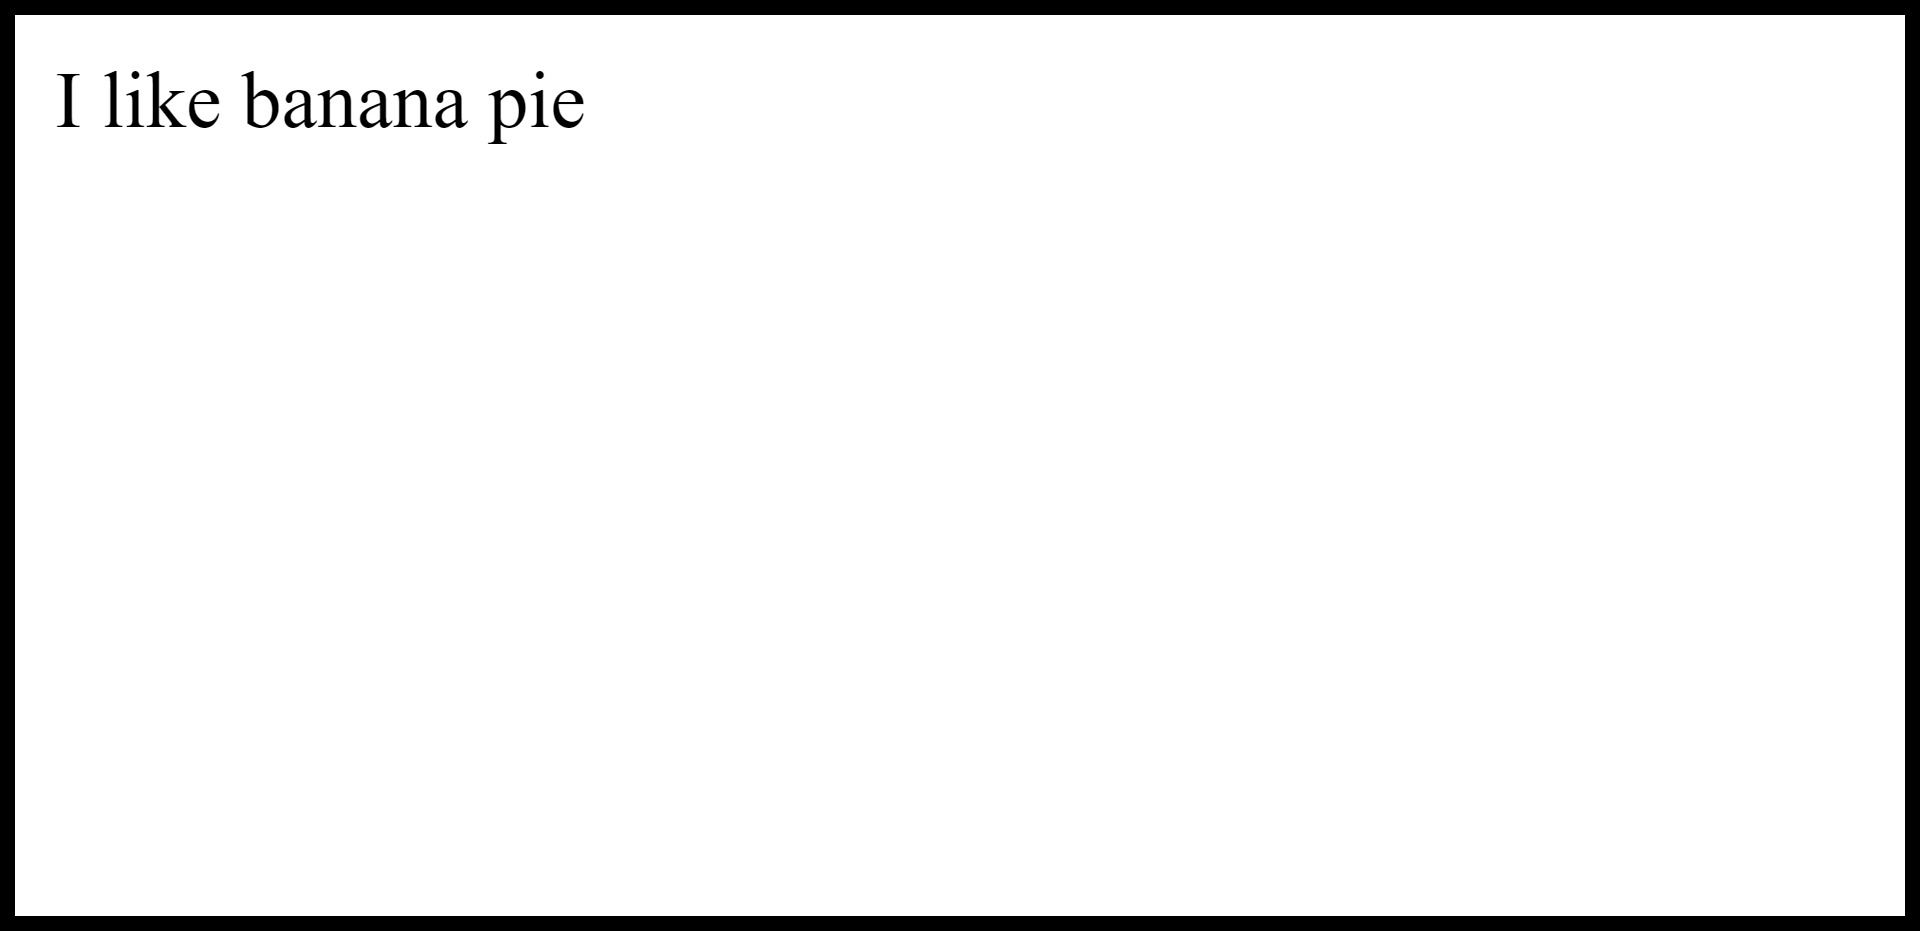
\includegraphics[width=.85\textwidth]{images/figures/fig5.3.png} \\ The RegEx allows us to check a specific pattern of string that we can replace with a function with another string.
        \item - \\ \includegraphics[width=.85\textwidth]{images/figures/fig5.4.png} \\ The RegEx allows us to check a pattern that begin with the sequence of letters 'go' and end with the sequence of letters 'd' wheter or not there is a letter or sequence of letters between them.
        
        \newpage

        \item - \\ \includegraphics[width=.85\textwidth]{images/figures/fig5.5.png} \\ The RegEx allows us to check a pattern that begin with the sequence of letters 'go' and end with the sequence of letters 'd' wheter or not there is a letter between them.
        \item - \\ \includegraphics[width=.85\textwidth]{images/figures/fig5.6.png} \\ The RegEx allows us to check a pattern that begin with the sequence of letter 'go' and end with the sequence of letter 'd' wheter or not there is a sequence of letters between them in a min and max range amount of letters set by the n as min and m as max. in this case i use {2,3}
    \end{enumerate}

    \newpage

    \item -   
    \begin{enumerate}
        \item - \\ 
        \includegraphics[width=.85\textwidth]{images/figures/fig6.1_a.png} \\ 
        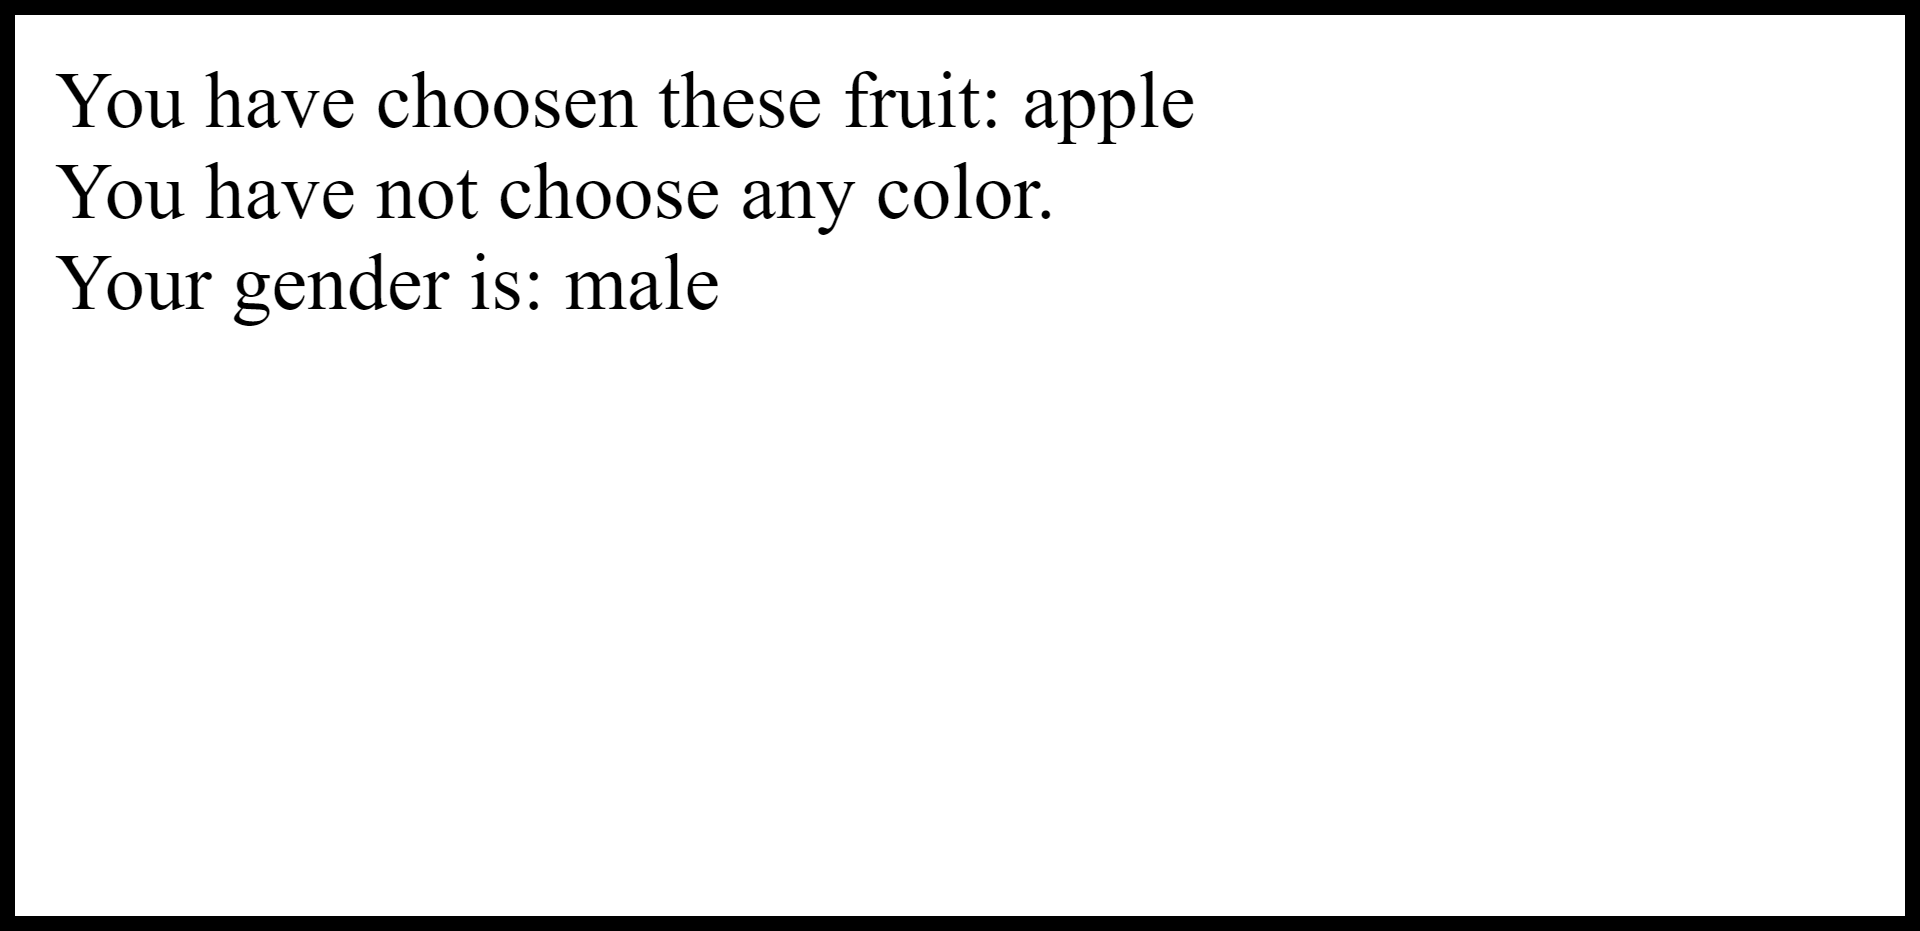
\includegraphics[width=.85\textwidth]{images/figures/fig6.1_b.png} \\ 
        The form switches page when the submit button is pressed

        \newpage

        \item - \\ \includegraphics[width=.85\textwidth]{images/figures/fig6.2.png} \\ The form doesnt switch page since the JQuery grap the response of the proccess file
    \end{enumerate}
\end{enumerate}

\end{document}